\documentclass{article}
\usepackage[margin=2.8cm]{geometry}

\usepackage[table]{xcolor}
\usepackage{tikz}
\usetikzlibrary{shapes,arrows,arrows.meta,positioning,fit,calc,decorations.pathmorphing,backgrounds,patterns}

\usepackage{amsmath,amssymb}
\usepackage{mathtools}
\usepackage{xspace}

\usepackage[noend]{algpseudocode}
\usepackage{amsthm}
\usepackage{cleveref}

\usepackage{float}
\usepackage{boxedminipage}
\usepackage{hyperref}

\usepackage{tcolorbox}
\tcbuselibrary{skins,breakable}

% --- Symbols (mirroring fresh_simplex_with_notarizations.tex) ---
\newcommand{\genesis}{\ensuremath{B_{\mathrm{gen}}}}
\newcommand{\T}{\ensuremath{\mathcal{T}}}
\newcommand{\slot}{\operatorname{\mathrm{slot}}}

\newcommand{\target}{\mathsf{target}}
\newcommand{\kind}{\mathsf{kind}}
\newcommand{\height}{\mathsf{height}}
\newcommand{\validator}{\mathsf{validator}}
\newcommand{\just}{\ensuremath{\mathsf{justify}}\xspace}
\newcommand{\notar}{\ensuremath{\mathsf{notarize}}\xspace}
\newcommand{\parent}{\mathsf{parent}}

\newcommand{\finalizeHeight}{\mathsf{finalize\_height}}
\newcommand{\finalizeTarget}{\mathsf{finalize\_target}}
\newcommand{\jtargets}{\mathsf{jtargets}}
\newcommand{\ntargets}{\mathsf{ntargets}}
\newcommand{\nslots}{\mathsf{nslots}}
\newcommand{\penalties}{\mathsf{penalties}}
\newcommand{\fresh}{\mathsf{fresh}}
\newcommand{\hash}{\mathsf{hash}}
\newcommand{\key}{\mathsf{key}}
\newcommand{\bit}{\mathsf{bit}}
\newcommand{\currentSlot}{\mathsf{currentSlot}}
\newcommand{\start}{\mathsf{start}}
\newcommand{\vote}{\mathsf{vote}}
\newcommand{\syncer}{\mathsf{syncer}}

\newcommand{\GST}{\ensuremath{\mathsf{GST}}}
\newcommand{\OHM}{online-honest majority\xspace}
\newcommand{\HAP}{honest available-chain proposer\xspace}
\newcommand{\HAR}{honest available-chain relay\xspace}
\newcommand{\AHA}{all-honest-awake\xspace}

\newcommand{\processSlot}{\textsf{processSlot}\xspace}
\newcommand{\processBlock}{\textsf{processBlock}\xspace}
\newcommand{\processHeight}{\textsf{processHeight}\xspace}
\newcommand{\processVote}{\textsf{processVote}\xspace}
\newcommand{\processInactivityPenalties}{\textsf{processInactivityPenalties}\xspace}
\newcommand{\constructVote}{\textsf{constructVote}\xspace}
\newcommand{\onBlock}{\textsf{onBlock}\xspace}
\newcommand{\updateForkChoiceRoot}{\textsf{updateForkChoiceRoot}\xspace}
\newcommand{\updateRootInSlot}{\textsf{updateRootInSlot}\xspace}
\newcommand{\updateRootFromVotes}{\textsf{updateRootFromVotes}\xspace}
\newcommand{\onViewMerge}{\textsf{onViewMerge}\xspace}
\newcommand{\updateFinalized}{\textsf{updateFinalized}\xspace}
\newcommand{\getConfirmed}{\textsf{getConfirmed}\xspace}
\newcommand{\newKey}{\mathsf{newKey}}

\newcommand{\comm}[1]{\bar{#1}}

\algdef{SE}[EVENT]{Event}{EndEvent}[1]{\textbf{at}\ #1\ \algorithmicdo}{\algorithmicend\ \textbf{event}}
\algtext*{EndEvent}
\algrenewcommand\textproc{}

% --- Flag macro for simplification caveats ---
\newcommand{\flag}[1]{%
  \par\smallskip\noindent\textcolor{red}{$\blacktriangleright$ \textbf{Flag.}~\textit{#1}}\par\smallskip}

% --- Intuition box ---
\newtcolorbox{intuition}[1][]{
  colback=blue!4!white,
  colframe=blue!40!black,
  boxrule=0.4pt,
  arc=2pt,
  left=2mm,right=2mm,top=1.5mm,bottom=1.5mm,
  fonttitle=\bfseries,
  title={Intuition},
  #1
}

% --- Theorem environments ---
\theoremstyle{plain}
\newtheorem{theorem}{Theorem}
\newtheorem{corollary}[theorem]{Corollary}
\newtheorem{lemma}[theorem]{Lemma}
\newtheorem{proposition}[theorem]{Proposition}
\newtheorem{property}[theorem]{Property}

\theoremstyle{definition}
\newtheorem{definition}[theorem]{Definition}

\theoremstyle{remark}
\newtheorem{remark}[theorem]{Remark}

\renewcommand{\paragraph}[1]{\vspace{6pt}\noindent\textbf{#1}}

\title{Fresh Simplex with Prefix Notarizations\\
\large \textit{simplified, intuition-first}}
\author{}
\date{}

\begin{document}
\maketitle

\begin{abstract}
\noindent A simplified, intuition-first companion to \texttt{fresh\_simplex\_with\_notarizations.tex}. All definitions and theorem statements are preserved verbatim. Long case-by-case proofs are replaced by sketches that highlight the core argument; full proofs live in the original. Diagrams illustrate the key mechanisms. Items in red (\textcolor{red}{$\blacktriangleright$~\textbf{Flag}}) mark places where the simplified treatment glosses over a subtlety.
\end{abstract}

\tableofcontents
\medskip\hrule\medskip

\section{Setup}\label{sec:setup}

There are $n$ validators, of which at most $f$ are adversarial. We assume $n \geq 3f + 1$. A \emph{quorum} is any set of $\geq 2n/3$ validators. Any two quorums intersect in at least $n/3 + 1 > f$ validators, so their intersection always contains an honest validator.

\begin{definition}[Block, chain]\label{def:block}
A \emph{block} $B$ has a \emph{parent} block, a \emph{slot} $B.\slot$, and a set of votes (Definition~\ref{def:vote}). The genesis block $\genesis$ has no parent and slot $0$. Slots strictly increase along parent links: $B.\slot > B.\parent.\slot$. Blocks form a tree rooted at $\genesis$. Write $B \preceq B'$ when $B$ is an ancestor of $B'$ (or $B = B'$), and $B \sim B'$ (\emph{compatible}) when $B \preceq B'$ or $B' \preceq B$. Two chains \emph{conflict} when their tips are not compatible.
\end{definition}

\paragraph{Two counters: slot vs.\ height.} The \emph{slot} $B.\slot$ is a chain-position counter set by the proposer (strictly increasing along parent links). The \emph{height} $h$ is a finality-gadget counter, advanced once per \emph{cert event} on a chain --- by a $\geq 2n/3$ quorum. Slots and heights are not in lockstep: a single height can span many slots.

\begin{definition}[Height]\label{def:height}
\emph{Height} is the finality-gadget counter, separate from slot. The genesis height is $0$; height advances by exactly $1$ via fixed-target justification (Definition~\ref{def:just}) or prefix notarization (Definition~\ref{def:notar}).
\end{definition}

\begin{definition}[Vote]\label{def:vote}
A \emph{vote} is a signed tuple
\[
  (\validator,\; \height,\; \slot,\; \target,\; \kind,\; \finalizeHeight,\; \finalizeTarget),
\]
with $\kind \in \{\just, \notar\}$ and $\target$ a block (never $\bot$). The pair $(\finalizeHeight, \finalizeTarget)$ is either both $\bot$ or a commitment to finalize a block at a height. A vote included on a chain must reference a target (and finalize target, when present) that exists on that chain.
\end{definition}

\subsection{Per-chain state}

For each chain $L$ we maintain a state $\sigma[L]$ tracking what the protocol has seen on that chain:
\[
  \sigma[L] = (L,\; s,\; h,\; s_h,\; \jtargets,\; \ntargets,\; \nslots,\; J,\; h_j,\; N,\; h_n,\; s_n,\; F,\; P).
\]
The fields used most often:
\begin{itemize}
  \item $s$: chain's current slot counter (\processSlot bumps it once per slot).
  \item $h$: current height; $s_h$ is the slot at which $h$ was last advanced on this chain.
  \item $\jtargets[i]$: target of $i$'s \just{} vote at the current height ($\bot$ if none seen).
  \item $\ntargets[i], \nslots[i]$: target and slot of $i$'s \emph{latest-slot} fresh vote at the current height, across both vote kinds.
  \item $J, h_j$: most recently justified block.
  \item $N, h_n, s_n$: most recently notarized block; $s_n$ is the common slot shared by the firing prefix-notarization quorum (zero on a justification advance, since justifications are bit-1 cert events).
  \item $F$: most recently finalized block.
  \item $P \subseteq \{1,\ldots,n\}$: validators who have signed a finalize commitment for $(J, h_j)$.
\end{itemize}
The genesis state has all maps empty, all heights/slots zero, and $L = J = N = F = \genesis$. We write $\sigma[L].h$, $\sigma[L].s_h$, etc., or simply drop the $L$ when unambiguous.

\begin{definition}[State-height]\label{def:sheight}
The \emph{state-height} of a block $B$ is $\sigma[B].h$: the height value after processing $B$ on its own chain.
\end{definition}

\section{Freshness, justification, notarization}\label{sec:fresh-just-notar}

\subsection{Height freshness}\label{sec:freshness}

A vote $v$ with target $T$ is processed on chain with head $L$ \emph{only if}
\[
  \sigma[L].h = v.\height \;\wedge\; T \preceq L \;\wedge\; T.\slot \geq \sigma[L].s_h.
\]

\begin{intuition}
The vote was cast at the current height ($v.\height = \sigma[L].h$), against an ancestor of $L$ ($T \preceq L$), that already lives in the height-$h$ window of $L$ ($T.\slot \geq s_h$). Equivalently (Remark~\ref{rem:fresh-equiv}), $T$'s own chain has reached state-height $h$. So a fresh vote attests: ``I saw $T$ as a chain that itself reached height $h$.''
\end{intuition}

\begin{remark}[Fresh window]\label{rem:fresh-equiv}
For $T \preceq L$, the slot bound $T.\slot \geq \sigma[L].s_h$ is equivalent to $\sigma[T].h = \sigma[L].h$.
\end{remark}

\begin{figure}[H]
\centering
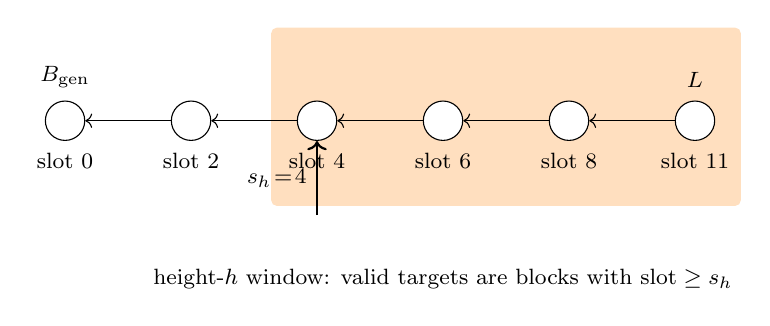
\begin{tikzpicture}[every node/.style={font=\footnotesize}]
  \foreach \i/\s/\name in {0/0/$\genesis$,1/2/,2/4/,3/6/,4/8/,5/11/$L$} {
    \node[draw, circle, minimum size=5mm, fill=white] (B\i) at (\i*1.6, 0) {};
    \node[below=1pt of B\i] {slot $\s$};
    \ifx&\name&\else
      \node[above=1pt of B\i] {\name};
    \fi
  }
  \foreach \i in {1,...,5} {
    \pgfmathtruncatemacro{\j}{\i-1}
    \draw[<-] (B\j) -- (B\i);
  }
  \begin{scope}[on background layer]
    \fill[orange!25, rounded corners=2pt]
      ([xshift=-4mm,yshift=-9mm]B2.south west) rectangle
      ([xshift=4mm,yshift=10mm]B5.north east);
  \end{scope}
  \draw[->, thick] (B2) ++(0,-12mm) -- (B2.south) node[midway, left, font=\footnotesize\itshape] {$s_h\!=\!4$};
  \node[below=15mm of B3, font=\footnotesize, align=center]
    {height-$h$ window: valid targets are blocks with $\slot \geq s_h$};
\end{tikzpicture}
\caption{The freshness window. Once height $h$ began at the block with slot $s_h$, only its descendants on $L$ are valid vote targets at height $h$.}\label{fig:freshness}
\end{figure}

\subsection{Justification and prefix notarization}

There are two ways to advance height by 1, both gated by a $\geq 2n/3$ fresh quorum.

\begin{definition}[Fixed-target justification]\label{def:just}
$T$ is \emph{justified at height $h$} on a chain with state $\sigma[L]$ ($\sigma[L].h = h$) iff
\[
  |\{i : \jtargets[i] = T\}| \geq 2n/3.
\]
Only \just{} votes with target \emph{exactly} $T$ contribute.
\end{definition}

\begin{definition}[Prefix notarization]\label{def:notar}
On chain $L$ at height $h$, $T$ is \emph{notarized at height $h$ with slot $s$} iff $T$ is the $\preceq$-maximum block such that some slot $s$ satisfies
\[
  |\{i : T \preceq \ntargets[i] \preceq L \;\wedge\; \nslots[i] = s\}| \geq 2n/3.
\]
\emph{Both} \just{} and \notar{} votes contribute via $\ntargets$ (latest-slot entry per validator), and the firing quorum must share a single $\nslots$ value $s$. When $T$ exists, the witnessing $s$ is unique (sets at distinct $s$ are disjoint and bounded by $n/3$). A justification of $T$ also fires a notarization at $T$: the justification branch sets $(J, N) \gets (T, T)$ jointly.
\end{definition}

\begin{figure}[H]
\centering
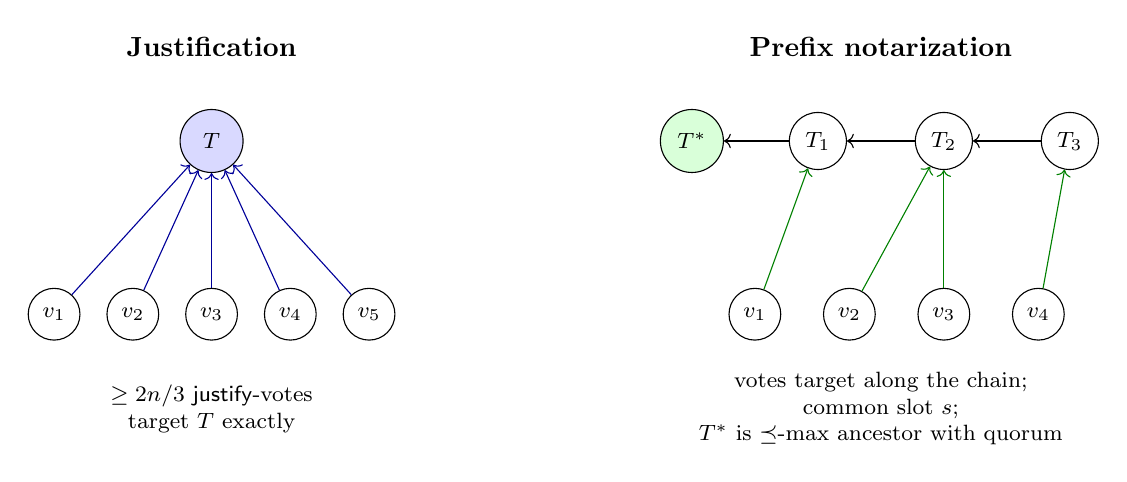
\begin{tikzpicture}[every node/.style={font=\footnotesize}]
  % Left: justification
  \begin{scope}
    \node[draw, circle, fill=blue!15, minimum size=8mm] (T) at (0, 0) {$T$};
    \foreach \i/\x in {1/-2,2/-1,3/0,4/1,5/2} {
      \node[draw, circle, minimum size=4mm] (V\i) at (\x, -2.2) {$v_\i$};
      \draw[->, blue!60!black] (V\i) -- (T);
    }
    \node[font=\bfseries] at (0, 1.2) {Justification};
    \node[align=center, font=\footnotesize] at (0, -3.4) {$\geq 2n/3$ \just{}-votes\\target $T$ exactly};
  \end{scope}
  % Right: prefix notarization
  \begin{scope}[xshift=8.5cm]
    \node[draw, circle, fill=green!15, minimum size=8mm] (Tstar) at (-2.4, 0) {$T^*$};
    \node[draw, circle, minimum size=7mm] (T1) at (-0.8, 0) {$T_1$};
    \node[draw, circle, minimum size=7mm] (T2) at (0.8, 0) {$T_2$};
    \node[draw, circle, minimum size=7mm] (T3) at (2.4, 0) {$T_3$};
    \draw[<-] (Tstar) -- (T1);
    \draw[<-] (T1) -- (T2);
    \draw[<-] (T2) -- (T3);
    \node[draw, circle, minimum size=4mm] (V1) at (-1.6, -2.2) {$v_1$};
    \node[draw, circle, minimum size=4mm] (V2) at (-0.4, -2.2) {$v_2$};
    \node[draw, circle, minimum size=4mm] (V3) at (0.8, -2.2) {$v_3$};
    \node[draw, circle, minimum size=4mm] (V4) at (2.0, -2.2) {$v_4$};
    \draw[->, green!50!black] (V1) -- (T1);
    \draw[->, green!50!black] (V2) -- (T2);
    \draw[->, green!50!black] (V3) -- (T2);
    \draw[->, green!50!black] (V4) -- (T3);
    \node[font=\bfseries] at (0, 1.2) {Prefix notarization};
    \node[align=center, font=\footnotesize] at (0, -3.4) {votes target along the chain;\\common slot $s$;\\$T^*$ is $\preceq$-max ancestor with quorum};
  \end{scope}
\end{tikzpicture}
\caption{Two height-advancing mechanisms. Justification needs all votes pinned to a single target. Prefix notarization tolerates a fan-out across descendants and pulls the firing block back to their deepest common ancestor; the common slot $s$ is what binds the contributors to a single chain (Lemma~\ref{lem:notar-unique-per-slot}).}\label{fig:just-notar}
\end{figure}

\paragraph{Why two mechanisms?} Justification is cleaner --- a single block, a bit-1 cert event --- but fragile under view shift: if validators see slightly different chain tips, no quorum forms on a single $T$. Prefix notarization is the resubmission fallback (R2 in the voting rule, \S\ref{sec:voting-rule}): even when validators target distinct descendants of a common ancestor, the prefix counting recovers a notarization of the ancestor. The shared slot $s$ is what guarantees safety: same-slot honest votes lie on a common chain (Lemma~\ref{lem:notar-unique-per-slot}).

\subsection{Finality and slashing}

\begin{definition}[Finality]\label{def:finality}
$J$ is \emph{finalized at height $h_j$} once $|P| \geq 2n/3$, where $P$ tracks validators that signed a vote committing $\finalizeHeight = h_j$, $\finalizeTarget = J$.
\end{definition}

\begin{definition}[Slashing rule E1]\label{def:slashing}
A validator is \emph{slashable} if it signed two votes $a, b$ (possibly $a = b$) with
\[
  b.\finalizeTarget \neq \bot \;\wedge\; a.\height = b.\finalizeHeight \;\wedge\; a.\target \neq b.\finalizeTarget.
\]
That is: a validator committing $(\finalizeHeight, \finalizeTarget) = (h_f, T_f)$ must not sign any vote at height $h_f$ with target $\neq T_f$.
\end{definition}

\begin{intuition}
There is exactly one slashing rule. Per-height \just{}-uniqueness is \emph{not} a slashing rule; honest validators avoid casting two \just{} votes at the same height behaviorally, via the voting rule (Definition~\ref{def:voting-rule}). A validator who never sets $\finalizeTarget \neq \bot$ is unconditionally non-slashable.
\end{intuition}

\subsection{State machine}\label{sec:state-machine}

The state machine has two per-chain routines: \processSlot, invoked once per slot on every maintained chain (even slots with no block), and \processBlock, additionally invoked when a block is processed. Height advances happen \emph{only} in \processSlot --- this means heights can advance even on empty slots, once enough votes have accumulated.

\begin{figure}[H]
\caption{State machine}\label{alg:state-machine}
\begin{center}
\begin{boxedminipage}{\textwidth}
\begin{algorithmic}[1]
\Function{\processSlot}{$\sigma$} \Comment{once per slot on every chain, even empty slots}
  \State $\sigma.s \gets \sigma.s + 1$
  \State $\sigma \gets \processHeight(\sigma)$; \Return $\sigma$
\EndFunction
\vspace{3pt}
\Function{\processBlock}{$\sigma,\; B$}
  \State \textbf{assert} $\sigma.s = B.\slot$ \Comment{caller advances $\sigma.s$ via \processSlot first}
  \State $\sigma.L \gets B$
  \For{each vote $v$ in $B$} $\sigma \gets \processVote(\sigma,\, v)$ \EndFor
  \State \Return $\sigma$
\EndFunction
\vspace{3pt}
\Function{\processVote}{$\sigma,\; v$}
  \State $i \gets v.\validator$
  \State $\fresh \gets (v.\height = \sigma.h) \land (v.\target \preceq \sigma.L) \land (v.\target.\slot \geq \sigma.s_h)$
  \If{$\fresh$ \textbf{and} $v.\slot > \sigma.\nslots[i]$}
    \State $\sigma.\ntargets[i] \gets v.\target$; \;\; $\sigma.\nslots[i] \gets v.\slot$
    \Comment{both kinds bump $\ntargets$, slot-gated}
  \EndIf
  \If{$\fresh$ \textbf{and} $v.\kind = \just$} \;
    $\sigma.\jtargets[i] \gets v.\target$
  \EndIf
  \If{$v.\finalizeHeight = \sigma.h_j$ \textbf{and} $v.\finalizeTarget = \sigma.J$} \;
    $\sigma.P \gets \sigma.P \cup \{i\}$
  \EndIf
  \State \Return $\sigma$
\EndFunction
\vspace{3pt}
\Function{\processHeight}{$\sigma$}
  \If{$|\sigma.P| \geq 2n/3$} \;\; $\sigma.F \gets \sigma.J$ \Comment{Finality}
  \EndIf
  \State $T \gets \arg\max_{T'} |\{i : \sigma.\jtargets[i] = T'\}|$ \Comment{$T \gets \bot$ if all $\bot$}
  \If{$T \neq \bot$ \textbf{and} $|\{i : \sigma.\jtargets[i] = T\}| \geq 2n/3$} \Comment{Justification (also a notarization)}
    \State $\sigma.J \gets T$, $\sigma.h_j \gets \sigma.h$, $\sigma.P \gets \emptyset$
    \State $\sigma.N \gets T$, $\sigma.h_n \gets \sigma.h$, $\sigma.s_n \gets 0$
    \State $\sigma.h \gets \sigma.h + 1$, $\sigma.s_h \gets \sigma.L.\slot$
    \State reset $\jtargets, \ntargets, \nslots$; \Return $\sigma$
  \EndIf
  \State $(B^*, s^*) \gets \arg\max_{\preceq}\,\bigl\{(B, s) : B \preceq \sigma.L \wedge |\{i : B \preceq \sigma.\ntargets[i] \preceq \sigma.L \wedge \sigma.\nslots[i] = s\}| \geq 2n/3\bigr\}$
  \If{$(B^*, s^*) \neq \bot$} \Comment{Prefix notarization fires}
    \State $\sigma.N \gets B^*$, $\sigma.h_n \gets \sigma.h$, $\sigma.s_n \gets s^*$
    \State $\sigma.h \gets \sigma.h + 1$, $\sigma.s_h \gets \sigma.L.\slot$
    \State reset $\jtargets, \ntargets, \nslots$
  \EndIf
  \State \Return $\sigma$
\EndFunction
\end{algorithmic}
\end{boxedminipage}
\end{center}
\end{figure}

\paragraph{Reading the algorithm.} \processHeight checks three branches \emph{in order}: (i) finality $F \gets J$ if $|P| \geq 2n/3$; (ii) justification on a single $T$; (iii) prefix notarization on the firing $(B^*, s^*)$. Branches (ii) and (iii) both advance height and reset $\jtargets, \ntargets, \nslots$; at most one fires per invocation. \processBlock never advances $h$ on its own --- height advances happen only in \processSlot, which the store calls on every slot.

\section{Accountable safety}\label{sec:safety}

The safety story is short: every height advance is gated by a $\geq 2n/3$ fresh quorum at height $h$, and finality at height $h$ is gated by a $\geq 2n/3$ finalize-quorum committing $(\finalizeHeight, \finalizeTarget) = (h, C)$. Quorum intersection and E1 then force any chain that reaches height $> h$ to extend $C$.

\begin{lemma}[Height progression]\label{lem:heightprog}
\processHeight increments $h$ by at most $1$ per invocation, and each increment is gated by a $\geq 2n/3$ quorum.
\end{lemma}

\begin{proof}[Proof]
Read off the algorithm: $h$ is updated only in the justification and notarization branches, each guarded by its $\geq 2n/3$ count. \qedhere
\end{proof}

\begin{lemma}[Checkpoint monotonicity]\label{lem:slotmono}
On any chain, $s, h, h_j, h_n, s_h, F, J, N$ are non-decreasing along $\preceq$, with $F \preceq J \preceq N$ at all times. Consequently, when $\sigma[Y].h = h$, the ancestors of $Y$ at state-height $h$ are exactly $\{B' \preceq Y : B'.\slot \geq \sigma[Y].s_h\}$.
\end{lemma}

\begin{proof}[Sketch]
$s$ only increases (in \processSlot); $h$ increases only by $1$ in the height-advance branches, which set $h_j, h_n \gets h$ and $s_h \gets L.\slot$. Slots strictly increase along $\preceq$, so $s_h$ is non-decreasing. $F$ updates only via $F \gets J$, so $F \preceq J$. The justification branch sets $J = N = T$ at the firing target; the notarization branch sets only $N \gets T$; freshness places the firing $T$ at slot $\geq s_h$, so by state-height monotonicity $T$ strictly succeeds the previous $N$. The interval claim follows from strict slot increase along $\preceq$ paired with state-height monotonicity.
\end{proof}

\begin{lemma}[Any chain past a finalized height contains the finalized block]\label{lem:mainsafety}
Unless $\geq n/3$ validators are slashable: if $C$ is finalized at height $h$, then $C \preceq B$ for every block $B$ with $\sigma[B].h > h$.
\end{lemma}

\begin{figure}[H]
\centering
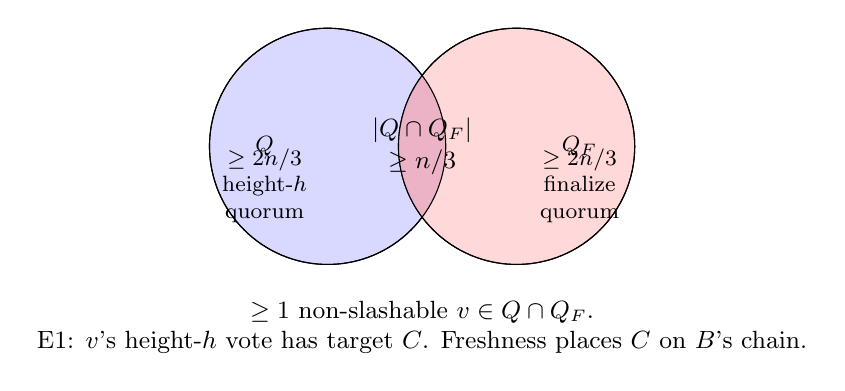
\begin{tikzpicture}[every node/.style={font=\footnotesize}]
  \begin{scope}
    \draw[fill=blue!15] (-1.2, 0) circle (1.5cm);
    \draw[fill=red!15] (1.2, 0) circle (1.5cm);
    \begin{scope}
      \clip (-1.2, 0) circle (1.5cm);
      \fill[purple!30] (1.2, 0) circle (1.5cm);
    \end{scope}
    \draw (-1.2, 0) circle (1.5cm);
    \draw (1.2, 0) circle (1.5cm);
    \node at (-2.0, 0) {$Q$};
    \node[align=center] at (-2.0, -0.5) {$\geq 2n/3$\\height-$h$\\quorum};
    \node at (2.0, 0) {$Q_F$};
    \node[align=center] at (2.0, -0.5) {$\geq 2n/3$\\finalize\\quorum};
    \node[font=\small\bfseries] at (0, 0.2) {$|Q \cap Q_F|$};
    \node[font=\small] at (0, -0.2) {$\geq n/3$};
  \end{scope}
  \node[align=center, font=\small] at (0, -2.3)
    {$\geq 1$ non-slashable $v \in Q \cap Q_F$.\\E1: $v$'s height-$h$ vote has target $C$. Freshness places $C$ on $B$'s chain.};
\end{tikzpicture}
\caption{Safety via quorum intersection. The non-slashable validator in $Q \cap Q_F$ is forced by E1 to vote at height $h$ for $C$, and by freshness this $C$ lies on the advancing chain.}\label{fig:safety}
\end{figure}

\begin{proof}[Sketch]
By Lemma~\ref{lem:heightprog} some $B^* \preceq B$ on $B$'s chain advanced height $h \to h+1$ via a fresh quorum $Q$ at height $h$. Finality of $C$ gives a quorum $Q_F$ committing $(\finalizeHeight, \finalizeTarget) = (h, C)$. Quorum intersection gives $|Q \cap Q_F| \geq n/3$, so a non-slashable $v \in Q \cap Q_F$ exists. By E1 (Definition~\ref{def:slashing}) on $v$'s votes in $Q$ and $Q_F$, $v$'s height-$h$ vote targets $C$. Freshness then places $C \preceq B^* \preceq B$.
\end{proof}

\begin{lemma}[Finalized blocks form a chain]\label{lem:finchain}
Unless $\geq n/3$ validators are slashable: any two finalized $(C, h), (C', h')$ are compatible, with $C \preceq C'$ when $h \leq h'$.
\end{lemma}

\begin{proof}[Sketch]
\emph{Same height $h = h'$:} $C'$'s finality requires a justification of $C'$ at $h$, giving a \just{}-quorum $Q'$ at target $C'$. Quorum intersection of $Q'$ with $C$'s finalize-quorum $Q_F$ gives a non-slashable $v$, and E1 forces $C = C'$.

\emph{Different heights $h < h'$:} let $Z$ be the chain on which $C'$ was finalized. Then $\sigma[Z].h \geq h' > h$, so Lemma~\ref{lem:mainsafety} gives $C \preceq Z$. Both $C, C'$ lie on $Z$, and $\sigma[C].h = h < h' = \sigma[C'].h$ (Remark~\ref{rem:fresh-equiv}), so state-height monotonicity forces $C \prec C'$.
\end{proof}

\begin{theorem}[Accountable safety]\label{thm:safety}
Unless $\geq n/3$ validators are slashable, no two conflicting blocks can be finalized.
\end{theorem}

\begin{proof}[Proof]
Immediate from Lemma~\ref{lem:finchain}.
\end{proof}

\begin{remark}[Ancestor notarizations are fine]\label{rem:notar-safety}
A prefix notarization at height $h$ on a chain containing a finalized $C$ may fire at an ancestor $T^* \preceq C$ (since \just{} votes also bump $\ntargets$). No per-chain invariant forces $N \succeq C$; the store (\S\ref{sec:store}) handles such cases via lex-max cert keys.
\end{remark}

\section{Fork-choice store}\label{sec:store}

A node tracks multiple chains. The \emph{store} is the per-node data structure that picks which chain to follow. It maintains a single \emph{root} block $R$ together with a cached \emph{cert key} $\key_R$. Whenever a height-advancing event (a \emph{cert event}) fires on any processed chain, the store compares its key against $\key_R$; on strict lex domination, $(R, \key_R)$ updates.

\subsection{Cert events and cert keys}

\begin{definition}[Cert event and cert key]\label{def:cert-event}
When \processHeight fires a height advance, the triggering event is a \emph{cert event}, characterized by:
\begin{itemize}
  \item the firing block $X = \sigma.N$ (the justified target $T$ in branch (ii); the prefix-notar endpoint $T^*$ in branch (iii));
  \item the height $h$ at which the advance fires;
  \item a \emph{bit} $b \in \{0, 1\}$: $b = 1$ for justification, $b = 0$ for prefix-notarization-only;
  \item the \emph{notarization slot} $s_n$: for $b = 0$, the common slot of the firing quorum; for $b = 1$, $s_n = 0$.
\end{itemize}
The \emph{cert key} is the lexicographic tuple
\[
  \key(X, h, b, s_n) \coloneqq (h,\; b,\; s_n,\; X.\slot,\; \hash(X)).
\]
\end{definition}

\begin{figure}[H]
\centering
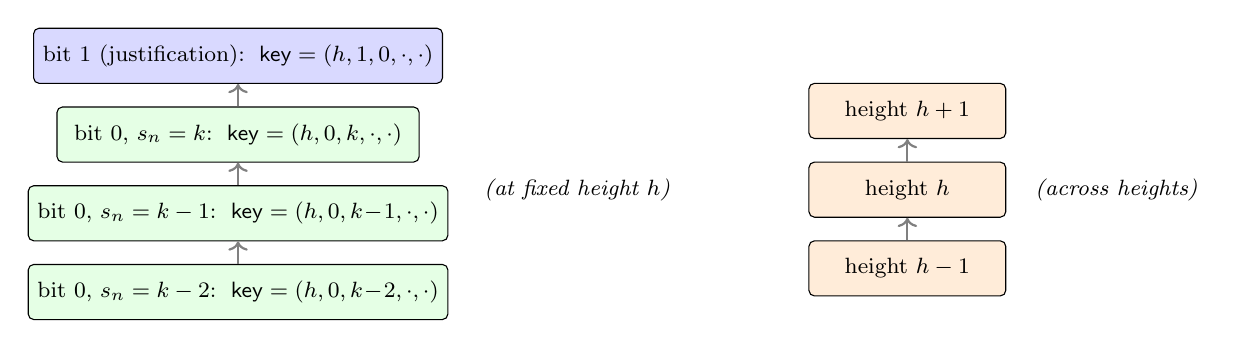
\begin{tikzpicture}[every node/.style={font=\footnotesize}]
  \node[draw, rounded corners=2pt, fill=blue!15, minimum width=4.6cm, minimum height=7mm]
    (J) at (0, 1.7) {bit $1$ (justification): $\,\key = (h, 1, 0, \cdot, \cdot)$};
  \node[draw, rounded corners=2pt, fill=green!10, minimum width=4.6cm, minimum height=7mm]
    (Nlate) at (0, 0.7) {bit $0$, $s_n = k$: $\,\key = (h, 0, k, \cdot, \cdot)$};
  \node[draw, rounded corners=2pt, fill=green!10, minimum width=4.6cm, minimum height=7mm]
    (Nmid) at (0, -0.3) {bit $0$, $s_n = k-1$: $\,\key = (h, 0, k\!-\!1, \cdot, \cdot)$};
  \node[draw, rounded corners=2pt, fill=green!10, minimum width=4.6cm, minimum height=7mm]
    (Nearly) at (0, -1.3) {bit $0$, $s_n = k-2$: $\,\key = (h, 0, k\!-\!2, \cdot, \cdot)$};
  \draw[->, thick, gray] (Nearly) -- (Nmid);
  \draw[->, thick, gray] (Nmid) -- (Nlate);
  \draw[->, thick, gray] (Nlate) -- (J);
  \node[anchor=west, font=\footnotesize\itshape] at (3.0, 0) {(at fixed height $h$)};

  % To the right: across heights
  \node[draw, rounded corners=2pt, fill=orange!15, minimum width=2.5cm, minimum height=7mm]
    (H1) at (8.5, -1) {height $h-1$};
  \node[draw, rounded corners=2pt, fill=orange!15, minimum width=2.5cm, minimum height=7mm]
    (H2) at (8.5, 0) {height $h$};
  \node[draw, rounded corners=2pt, fill=orange!15, minimum width=2.5cm, minimum height=7mm]
    (H3) at (8.5, 1) {height $h+1$};
  \draw[->, thick, gray] (H1) -- (H2);
  \draw[->, thick, gray] (H2) -- (H3);
  \node[anchor=west, font=\footnotesize\itshape] at (10, 0) {(across heights)};
\end{tikzpicture}
\caption{Cert-key lex order. At fixed height: bit 1 (justification) dominates any bit-0 cert; among bit-0 certs, larger $s_n$ dominates. Across heights: higher $h$ dominates everything below.}\label{fig:certkey}
\end{figure}

\paragraph{Why this ordering.} A justification is strictly more decisive than a notarization-only event: it pins a single target. So at the same height, bit-1 should dominate bit-0. Among bit-0 events, a more recent notarization slot reflects more current quorum agreement; older bit-0 certs are stale once a fresher one fires.

\subsection{Store and invariants}

\begin{definition}[Store]\label{def:store}
The store
\(
  \Sigma = (\sigma, \T, F, R, \key_R)
\)
holds: the state map $\sigma$ (per accepted block), the block tree $\T$, the store-finalized block $F$, the store root $R$, and the cached cert key $\key_R$. The genesis store has $\T = \{\genesis\}$, $F = R = \genesis$, and $\key_R = (0, 1, 0, \genesis.\slot, \hash(\genesis))$.
\end{definition}

The acceptance routine \onBlock takes a block $B$, runs \processSlot up to $B.\slot$ (so any pending cert event fires before $B$'s votes are folded in), then \processBlock. It then offers the post-state's two cert-event descriptors --- the justified $(\sigma[B].h_j, 1, \sigma[B].J, 0)$ and the notarized $(\sigma[B].h_n, 0, \sigma[B].N, \sigma[B].s_n)$ --- to \updateForkChoiceRoot. Each call updates $(R, \key_R)$ iff the descriptor's key strictly exceeds $\key_R$ and $C \succeq F$ (so $R$ stays on the $F$-chain).

\begin{figure}[H]
\caption{Store and fork-choice}\label{alg:store}
\begin{center}
\begin{boxedminipage}{\textwidth}
\begin{algorithmic}[1]
\Function{\onBlock}{$\Sigma,\; B$}
  \State \textbf{assert} $B.\parent \in \Sigma.\T$ \textbf{and} $\Sigma.F \preceq B$
  \State $\Sigma.\T \gets \Sigma.\T \cup \{B\}$; \;\; $\sigma' \gets \Sigma.\sigma[B.\parent]$
  \While{$\sigma'.s < B.\slot$} $\sigma' \gets \processSlot(\sigma')$ \EndWhile
  \State $\sigma' \gets \processBlock(\sigma',\; B)$; \;\; $\Sigma.\sigma[B] \gets \sigma'$
  \State $\Sigma \gets \updateForkChoiceRoot(\Sigma,\; (\sigma'.h_j,\; 1,\; \sigma'.J,\; \sigma'.s_n))$ \Comment{Justified descriptor}
  \State $\Sigma \gets \updateForkChoiceRoot(\Sigma,\; (\sigma'.h_n,\; 0,\; \sigma'.N,\; \sigma'.s_n))$ \Comment{Notarized descriptor}
  \State $\Sigma \gets \updateFinalized(\Sigma,\; \sigma'.F)$
  \State \Return $\Sigma$
\EndFunction
\vspace{3pt}
\Function{\updateForkChoiceRoot}{$\Sigma,\; (h, b, C, s_n)$}
  \State $\newKey \gets (h, b, s_n, C.\slot, \hash(C))$
  \If{$\newKey > \Sigma.\key_R$ \textbf{and} $\Sigma.F \preceq C$}
    \State $\Sigma.R \gets C$; \;\; $\Sigma.\key_R \gets \newKey$
  \EndIf
  \State \Return $\Sigma$
\EndFunction
\vspace{3pt}
\Function{\updateFinalized}{$\Sigma,\; F_B$}
  \If{$F_B \succ \Sigma.F$ \textbf{and} $F_B \preceq \Sigma.R$}
    \State $\Sigma.F \gets F_B$
  \EndIf
  \State \Return $\Sigma$
\EndFunction
\vspace{3pt}
\Function{\getConfirmed}{$\Sigma,\; \Omega$}
  \State \Return any block in $\Sigma.\T$ that descends from $\Sigma.R$ (chosen via auxiliary state $\Omega$)
\EndFunction
\end{algorithmic}
\end{boxedminipage}
\end{center}
\end{figure}

\paragraph{$\Omega$, the auxiliary state.} The protocol fixes only that $\getConfirmed$ returns a descendant of $\Sigma.R$. It does not constrain how $\Omega$ disambiguates among descendants. Different validators may pass different $\Omega$, and a single validator may pass different $\Omega$ at different call sites.

\subsection{Unconditional invariants}

\begin{lemma}[Root-key monotonicity]\label{lem:Rs-key-monotone}
$\Sigma.\key_R$ is non-decreasing over time.
\end{lemma}

\begin{proof}[Proof] \updateForkChoiceRoot only ever raises $\key_R$ via its strict guard. \end{proof}

\begin{theorem}[Local irreversibility of finality]\label{thm:finperm}
Once $\Sigma.F = F$, the store-finalized block is always a descendant of $F$.
\end{theorem}

\begin{proof}[Proof] \updateFinalized's guard $F_B \succ \Sigma.F$ forces strict $\preceq$-extension. \end{proof}

\begin{theorem}[$F \preceq R$]\label{thm:fleqr}
The store maintains $F \preceq R$ at all times.
\end{theorem}

\begin{proof}[Proof]
By induction. At genesis, $F = R = \genesis$. \updateForkChoiceRoot replaces $R$ only with a $C \succeq F$, preserving the invariant. \updateFinalized's guard $F_B \preceq R$ ensures the new $F$ stays $\preceq R$.
\end{proof}

\begin{remark}[$\Sigma.F$ is finalized somewhere]\label{rem:fs-invariant}
$\Sigma.F$ is either $\genesis$ or a block that was finalized on some chain --- $\Sigma.F$ only advances via \updateFinalized to $\sigma[B].F$, and $\sigma[B].F \neq \genesis$ requires the finality branch of \processHeight to have fired on $B$'s chain. Moreover, when $(J, h_j)$ has been justified on some chain, the descriptor $(h_j, 1, J, 0)$ was offered to \updateForkChoiceRoot, so $\key_R \geq (h_j, 1, 0, J.\slot, \hash(J))$ for every such pair with $J \succeq \Sigma.F$.
\end{remark}

\begin{theorem}[Fork-choice consistency]\label{thm:fcconsistency}
Once $\Sigma.F = F$, $\getConfirmed(\Sigma, \Omega)$ descends from $F$ at all future times, for every $\Omega$.
\end{theorem}

\begin{proof}[Proof] $F \preceq \Sigma.F \preceq \Sigma.R$ (Theorems~\ref{thm:finperm},~\ref{thm:fleqr}); $\getConfirmed$ returns a descendant of $\Sigma.R$. \end{proof}

\begin{figure}[H]
\centering
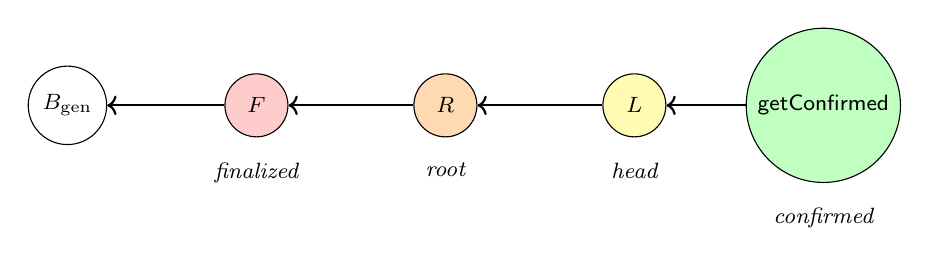
\begin{tikzpicture}[every node/.style={font=\footnotesize}]
  \foreach \i/\name/\fill in {0/$\genesis$/white,1/$F$/red!20,2/$R$/orange!30,3/$L$/yellow!30,4/$\getConfirmed$/green!25} {
    \node[draw, circle, minimum size=8mm, fill=\fill] (B\i) at (\i*2.4, 0) {\name};
  }
  \foreach \i in {1,...,4} {
    \pgfmathtruncatemacro{\j}{\i-1}
    \draw[<-, thick] (B\j) -- (B\i);
  }
  \node[below=2mm of B1, align=center, font=\footnotesize\itshape] {finalized};
  \node[below=2mm of B2, align=center, font=\footnotesize\itshape] {root};
  \node[below=2mm of B3, align=center, font=\footnotesize\itshape] {head};
  \node[below=2mm of B4, align=center, font=\footnotesize\itshape] {confirmed};
\end{tikzpicture}
\caption{Store-chain invariant: $F \preceq R \preceq \getConfirmed$ on the canonical chain. $F$ is irreversible once set.}\label{fig:store-chain}
\end{figure}

\subsection{Properties under $f < n/3$}

The remaining store properties --- key for inter-node consistency and lock-in --- assume $< n/3$ validators are slashable.

\begin{lemma}[Checkpoint chain]\label{lem:certchain}
Unless $\geq n/3$ slashable: if $F$ is finalized at height $h_F$ and a cert event $(C, h, b)$ fired on any processed chain with $h \geq h_F$, then $F \sim C$, with $F \prec C$ when $h > h_F$.
\end{lemma}

\begin{proof}[Sketch]
The cert event fired at the post-state of some processed block $B$ with $\sigma[B].h \geq h+1 > h_F$, so $C \preceq B$ and Lemma~\ref{lem:mainsafety} gives $F \preceq B$, hence $F \sim C$. For $h > h_F$, state-height monotonicity on the comparable pair forces $F \prec C$.
\end{proof}

\begin{lemma}[Upgrade]\label{lem:upgrade}
Unless $\geq n/3$ slashable: if $F$ is finalized at $h_F$ and the node has processed some block whose post-state has $(F, h_F)$ as its justified checkpoint, then $R \succeq F$ at all future times.
\end{lemma}

\begin{proof}[Sketch]
At the moment $\onBlock$ offers the descriptor $(h_F, 1, F, 0)$, let $F^0 = \Sigma.F$. If $F \preceq F^0$, $\Sigma.R \succeq \Sigma.F \succeq F$ already (Theorem~\ref{thm:fleqr}). Else $F^0 \preceq F$, so the filter passes and $\key_R \geq (h_F, 1, 0, F.\slot, \hash(F))$. Subsequent $\key_R$-monotonicity preserves this. If a later cert event fires at height $> h_F$, Lemma~\ref{lem:certchain} gives $F \prec R$. If at height $h_F$ with bit 1, justification of $\neq F$ would intersect $F$'s finalize-quorum at a non-slashable validator and force equality by E1.
\end{proof}

\begin{theorem}[Lock-in]\label{thm:lockin}
Unless $\geq n/3$ slashable: once a node processes a block whose post-state has $(F, h_F)$ as its justified checkpoint, $R \succeq F$ persists, and $\getConfirmed(\Sigma, \Omega)$ always returns a descendant of $F$.
\end{theorem}

\begin{proof}[Proof]
Lemma~\ref{lem:upgrade} gives $R \succeq F$; $\getConfirmed$ descends from $R$ for every $\Omega$.
\end{proof}

\begin{theorem}[Local acceptance of finality updates]\label{thm:finlive}
Unless $\geq n/3$ slashable: if $\onBlock(B)$'s post-state has finalized block $F_B$, then after processing $\Sigma.F \succeq F_B$.
\end{theorem}

\begin{proof}[Sketch]
If $\Sigma.F \succeq F_B$ already, done. Otherwise Lemma~\ref{lem:finchain} gives $\Sigma.F \prec F_B$; some ancestor $B' \preceq B$ had post-state-justified $(F_B, h_{F_B})$, so by lock-in (Lemma~\ref{lem:upgrade}) $R \succeq F_B$, and \updateFinalized's guard passes.
\end{proof}

\begin{theorem}[Order independence]\label{thm:orderindep}
Unless $\geq n/3$ slashable: the store state after processing a set of blocks depends only on the set, not the order.
\end{theorem}

\begin{proof}[Sketch]
$\sigma$ is a deterministic per-block recursion, so depends only on the processed set. $F$ converges to the maximum finalized block in the set (Lemma~\ref{lem:finchain} gives a chain; Theorem~\ref{thm:finlive} pulls $F$ up to it). $R$ is the lex-max over the multiset of cert descriptors offered, which is itself determined by the processed set; descriptors below $\key(F_{\max}, \cdot)$ are dominated, and any competitive descriptor at height $h_{F_{\max}}$ with bit 1 must coincide with $F_{\max}$ by quorum-intersection + E1.
\end{proof}

\begin{corollary}[Cross-node agreement]\label{cor:agreement}
Unless $\geq n/3$ slashable: nodes that have processed the same set of blocks have identical $(\sigma, \T, F, R, \key_R)$.
\end{corollary}

\begin{lemma}[Cached key dominates every cert event]\label{lem:Rs-key-dominates}
Unless $\geq n/3$ slashable: every cert event $(X, h, b, s_n)$ that has fired on any processed chain satisfies $\key(X, h, b, s_n) \leq \Sigma.\key_R$.
\end{lemma}

\begin{proof}[Sketch]
Three cases at the moment the descriptor was offered, with $F^0 = \Sigma.F$ and $h_{F^0}$ its finalized height. If $h > h_{F^0}$, the filter passes (Lemma~\ref{lem:certchain}); $\key_R$ rises to $\geq \key$. If $h = h_{F^0}$ and $b = 0$, the cached bit-1 from $F^0$'s prior justification dominates. If $h = h_{F^0}$ and $b = 1$, justification of $X$ at $h_{F^0}$ + finality of $F^0$ at $h_{F^0}$ + E1 force $X = F^0$. If $h < h_{F^0}$, $\key_R$ already dominates on the leading coordinate.
\end{proof}

\begin{corollary}[No cert above the root]\label{cor:no-high-cert}
Unless $\geq n/3$ slashable: every cert event $(X, h, b, s_n)$ has $h \leq R.h$.
\end{corollary}

\begin{corollary}[Processed-block height bound]\label{cor:processed-height-bound}
Unless $\geq n/3$ slashable: every processed block $B$ satisfies $\sigma[B].h \leq R.h + 1$.
\end{corollary}

\begin{proof}[Proof] If $\sigma[B].h \geq 1$, the most recent height advance leading to $\sigma[B].h$ is a cert event at height $\sigma[B].h - 1$; Corollary~\ref{cor:no-high-cert} bounds it by $R.h$. \end{proof}

\section{Inactivity leak}\label{sec:leak}

The leak section extends the per-chain state with a non-negative penalty counter $\sigma.\penalties[i]$ and a transition function \processInactivityPenalties invoked each slot by an extended \processSlot. The other algorithms (\processBlock, \processVote, \processHeight) are unchanged.

\subsection{Penalty layers}

\begin{figure}[H]
\caption{Penalty extension}\label{alg:leak-processslot}
\begin{center}
\begin{boxedminipage}{\textwidth}
\begin{algorithmic}[1]
\Function{\processSlot}{$\sigma$} \Comment{extended: tracks penalties}
  \State $\sigma.s \gets \sigma.s + 1$; \;\; $\sigma_{\mathrm{pre}} \gets \sigma$
  \State $\sigma \gets \processHeight(\sigma)$; \;\; $\sigma \gets \processInactivityPenalties(\sigma_{\mathrm{pre}}, \sigma)$
  \State \Return $\sigma$
\EndFunction
\vspace{3pt}
\Function{\processInactivityPenalties}{$\sigma_{\mathrm{pre}}, \sigma_{\mathrm{post}}$}
  \If{$\sigma_{\mathrm{pre}}.h = \sigma_{\mathrm{post}}.h$} \Comment{Layer 1: stall}
    \For{each $i$ with $\sigma_{\mathrm{post}}.\ntargets[i] = \bot$} bump $\sigma_{\mathrm{post}}.\penalties[i]$ \EndFor
  \EndIf
  \If{$\sigma_{\mathrm{pre}}.J = \sigma_{\mathrm{post}}.J$} \Comment{Layer 2 target}
    \State $T^* \gets$ plurality target across $\sigma_{\mathrm{pre}}.\jtargets$ (deterministic tiebreak; $\bot$ if all $\bot$)
    \For{each $i$ with $\sigma_{\mathrm{pre}}.\jtargets[i] \neq T^*$ \textbf{or} $\bot$} bump $\sigma_{\mathrm{post}}.\penalties[i]$ \EndFor
  \EndIf
  \If{$\sigma_{\mathrm{pre}}.F = \sigma_{\mathrm{post}}.F$ \textbf{and} $\sigma_{\mathrm{pre}}.F \prec \sigma_{\mathrm{pre}}.J$} \Comment{Layer 2 finalize}
    \For{each $i \notin \sigma_{\mathrm{pre}}.P$} bump $\sigma_{\mathrm{post}}.\penalties[i]$ \EndFor
  \EndIf
  \State \Return $\sigma_{\mathrm{post}}$
\EndFunction
\end{algorithmic}
\end{boxedminipage}
\end{center}
\end{figure}

\paragraph{Three independent layers.} \emph{Layer 1 (stall):} fires when no height advance fired this slot --- bump every validator who hasn't cast a fresh vote yet at the current height. \emph{Layer 2 target:} fires when the justification branch did not advance --- bump everyone whose \jtargets entry isn't on the plurality target (so $> n/3$ are bumped, since the plurality is $< 2n/3$). \emph{Layer 2 finalize:} fires when finality is pending and didn't advance --- bump everyone not in $P$ (so $> n/3$ are bumped).

\subsection{Tightness}

\begin{definition}[Non-finality period]\label{def:non-fin-period}
A maximal interval of consecutive slots on a chain in which $F$ does not advance. Each slot is one of: \emph{pending-stuck} ($F \prec J$ at slot start), \emph{stable-stuck} ($F = J$ and $J$ does not advance), or \emph{transition} ($F = J$ and $J$ advances at the slot, opening a gap).
\end{definition}

\begin{theorem}[Non-finality period penalty bound]\label{thm:tightness}
Over any non-finality period of length $T \geq 1$ on any chain, the total penalty increment across all validators is at least $(T - 1) \cdot n/3$.
\end{theorem}

\begin{proof}[Sketch]
At most one transition slot per period: after a transition, $J$ has advanced past the period's frozen $F$, so all subsequent slots are pending-stuck. Each pending-stuck slot fires Layer-2-finalize ($> n/3$ bumped); each stable-stuck slot fires Layer-2-target ($> n/3$ bumped). Summing across $T-1$ such slots gives $> (T-1)\cdot n/3$.
\end{proof}

\subsection{Honest voting rule}\label{sec:voting-rule}

\begin{figure}[H]
\caption{Honest voting rule}\label{alg:voting-rule}
\begin{center}
\begin{boxedminipage}{\textwidth}
\begin{algorithmic}[1]
\Function{\constructVote}{$V, \Sigma, \Omega$}
  \State $T \gets \getConfirmed(\Sigma, \Omega)$; \;\; $h_c \gets \sigma[T].h$; \;\; $h_j \gets \sigma[T].h_j$; \;\; $J \gets \sigma[T].J$
  \vspace{3pt}
  \State \textbf{-- Target --}
  \If{$\exists v \in V$ with $v.\finalizeHeight = h_c$ and $v.\finalizeTarget \neq \bot$}
    \State $T_c \gets v.\finalizeTarget$ \Comment{$i$ is locked at $h_c$}
  \Else
    \State $T_c \gets T$ \Comment{unlocked}
  \EndIf
  \vspace{3pt}
  \State \textbf{-- Vote kind \& finalize --}
  \If{$\nexists v \in V$ with $v.\height = h_c$} \Comment{first vote at $h_c$ (R1): \just{}}
    \If{every $v \in V$ with $v.\height = h_j$ has $v.\target = J$}
      \State $(f_h, f_t) \gets (h_j, J)$
    \Else
      \State $(f_h, f_t) \gets (\bot, \bot)$
    \EndIf
    \State \Return $(i, h_c, \currentSlot, T_c, \just, f_h, f_t)$
  \Else \Comment{already voted at $h_c$ (R2): \notar{} resubmission}
    \State \Return $(i, h_c, \currentSlot, T_c, \notar, \bot, \bot)$
  \EndIf
\EndFunction
\end{algorithmic}
\end{boxedminipage}
\end{center}
\end{figure}

\paragraph{Two branches.} (R1) fires once per height: it casts the \just{} vote and may attach a finalize commitment to $(h_j, J)$ \emph{provided} every prior vote of $i$ at height $h_j$ already targeted $J$ (else attach $(\bot, \bot)$ to stay E1-safe). (R2) is the resubmission: at every later voting opportunity while canonical stays at $h_c$, cast a \notar{} vote on the current canonical target. Two prior votes at $h_c$ cannot disagree on target if a finalize lock is in force --- target selection forces $T_c = $ the locked finalize target.

\paragraph{Why check ``every'' prior $h_j$-vote.} A locked R2 at height $h_j$ may have chosen a different target than the original R1, due to a view shift between the two firings. Committing $f_t = J$ at $h_j$ then would violate E1 against that R2. The conditional refuses the commitment in that case --- $i$ misses this finalization opportunity but stays slashing-free.

\begin{lemma}[Honest E1 safety]\label{lem:honest-e1}
A validator following Definition~\ref{def:voting-rule} never produces an E1-violating pair.
\end{lemma}

\begin{proof}[Sketch]
The finalize-bearing $v_2$ comes from R1 with $(f_h, f_t) = (h_j, J)$ read from canonical. If $v_1$ was cast \emph{before} $v_2$, the (R1) finalize-conditional fired only because every prior $h_j$-vote targeted $J$, so $v_1.\target = J$. If $v_1$ was cast \emph{after} $v_2$, the lock at $h_c = h_*$ in target selection forces $v_1.\target = T_*$. The diagonal case ($v_1 = v_2$) is vacuous since $h_c \neq h_j$.
\end{proof}

\subsection{Layer-1 fairness}

The fairness theorem says: an honest validator's vote, once included on any extension of its canonical chain still at the same state-height, exempts it from Layer-1 penalties for as long as state-height stays put.

The proof factors through four supporting facts:

\begin{lemma}[Per-height \just{}-uniqueness]\label{lem:just-unique-height}
If $f < n/3$ and honest validators follow Definition~\ref{def:voting-rule}: any two blocks justified at the same height (on any chains processed by the node) coincide.
\end{lemma}

\begin{proof}[Sketch] Each justification gives a $\geq 2n/3$ \just{}-quorum at that height; intersection gives $\geq n/3$ shared signers. Some shared signer is honest; by R1 the honest validator emits at most one \just{} vote per height, so the two targets coincide. \end{proof}

\begin{lemma}[Root-height notarize-only exclusivity]\label{lem:root-h-notarize-only}
Unless $\geq n/3$ slashable: if $\Sigma.\key_R.b = 0$, then no justification at height $\Sigma.\key_R.h$ has fired on any processed chain.
\end{lemma}

\begin{proof}[Sketch] If a justification $J_*$ at $h_R$ had fired, its descriptor would have been offered to \updateForkChoiceRoot. The filter $\Sigma.F \preceq J_*$ passes (using Lemma~\ref{lem:certchain} or, at $h_R = h_{F^0}$, E1 forces $F^0 = J_*$). So $\key_R$ rose to a bit-1 key at height $h_R$. By monotonicity (Lemma~\ref{lem:Rs-key-monotone}), the bit at $h_R$ stays $\geq 1$. \end{proof}

\begin{lemma}[Finalize lock implies prior justification cert]\label{lem:no-finalize-without-just}
If $i$ has cast a vote with $\finalizeTarget = T_f \neq \bot$ at $\finalizeHeight = h'$, then $T_f$ was justified at $h'$ on some processed chain by the time of casting.
\end{lemma}

\begin{proof}[Sketch] Only R1 attaches a finalize commitment. The R1 conditional reads $(f_h, f_t) = (h_j, J)$ from canonical, which requires $\sigma[T_0].J = T_f$ for some canonical $T_0$ at $i$'s prior moment --- meaning the justification branch fired with target $T_f$ on that chain. \end{proof}

\begin{lemma}[Canonical-fresh honest vote]\label{lem:canonical-fresh-honest-vote}
Unless $\geq n/3$ slashable, and assuming $f < n/3$ with honest validators following Definition~\ref{def:voting-rule}: an honest $i$ with canonical $T$ and $h_c = \sigma[T].h$ produces a vote $v$ with $v.\target \preceq T$ and $\sigma[v.\target].h = h_c$. So $v$ is canonical-fresh on every extension $T' \succeq T$ with $\sigma[T'].h = h_c$.
\end{lemma}

\begin{proof}[Sketch]
$T$ descends from $R$ (Figure~\ref{alg:store}), with $\sigma[R].h = h_R \coloneqq \Sigma.\key_R.h$. State-height monotonicity bounds $h_c \in \{h_R, h_R + 1\}$. By the case split:
\begin{itemize}
\item \emph{$h_c = h_R + 1$:} a lock at $h_c$ would, by Lemma~\ref{lem:no-finalize-without-just}, require a justification at $h_c$ on some processed chain. But Lemma~\ref{lem:root-h-notarize-only}'s argument (transposed to height $h_c$) would have raised $\key_R.h$ to $h_c$, contradicting $\key_R.h = h_R$. So $i$ is unlocked: $T_c = T$.
\item \emph{$h_c = h_R$, $\bit_R = 0$:} no justification at $h_c$ has fired (Lemma~\ref{lem:root-h-notarize-only}); by Lemma~\ref{lem:no-finalize-without-just}, $i$ is unlocked: $T_c = T$.
\item \emph{$h_c = h_R$, $\bit_R = 1$:} if locked at $L$, Lemma~\ref{lem:no-finalize-without-just} gives $L$ justified at $h_c$ on some chain; $\bit_R = 1$ gives $R$ justified at $h_R = h_c$. Lemma~\ref{lem:just-unique-height} forces $L = R$, so $T_c = R \preceq T$.
\end{itemize}
In every case $\sigma[T_c].h = h_c$.
\end{proof}

\begin{theorem}[Layer-1 leak fairness]\label{thm:fairness}
Unless $\geq n/3$ slashable, and assuming $f < n/3$ with honest validators following Definition~\ref{def:voting-rule}: if honest $i$'s vote $v$ is included on any extension $T' \succeq T$ of its canonical chain with $\sigma[T'].h = h_c$, then for every slot processed on $T'$ with state-height still $h_c$, $i$'s Layer-1 increment on canonical is zero.
\end{theorem}

\begin{proof}[Sketch] Lemma~\ref{lem:canonical-fresh-honest-vote} makes $v$ canonical-fresh on $T'$, so processing $v$ sets $\ntargets[i] \neq \bot$. $\ntargets$ resets only at a height advance, which doesn't fire while state-height stays at $h_c$. Hence Layer-1 doesn't bump $i$. \end{proof}

\begin{remark}[Weakening $f < n/3$ for fairness]\label{rem:weak-fairness}
The $f < n/3$ assumption in Lemmas~\ref{lem:just-unique-height} and \ref{lem:canonical-fresh-honest-vote} can be replaced by ``$< n/3$ slashable'' if the slashing rules are extended with a double-\just-at-the-same-height rule (so two-target \just-quorums at the same height force every shared signer slashable).
\end{remark}

\section{Healing from asynchrony}\label{sec:healing}

This section gives the conditions under which the protocol \emph{heals} after a prolonged asynchronous period: starting from any honest local view, after a bounded number of synchronous slots with honest syncers, all honest $\getConfirmed$'s become pairwise compatible and monotone.

\subsection{Slot timing model}

\begin{definition}[Slots and voting time]\label{def:slots}
Time is partitioned into discrete slots indexed by $k$. Slot $k$ has start time $\start(k)$ with $\start(k+1) \geq \start(k) + 2\Delta$, and voting time $\vote(k) = \start(k) + \Delta$. Every honest validator $i$ invokes Definition~\ref{def:voting-rule} at $\vote(k)$ on its local store $\Sigma_i$.
\end{definition}

\begin{definition}[Syncer]\label{def:syncer}
A publicly known function $\syncer \colon \mathbb{N} \to \{1, \ldots, n\}$ assigns each slot $k$ a validator $\syncer(k)$. During the portion of slot $k$ before $\vote(k)$, $\syncer(k)$ runs the view-merge protocol (Appendix~\ref{app:view-merge}).
\end{definition}

\begin{definition}[View-merge guarantee]\label{ass:view-merge}
If $\syncer(k)$ is honest, all honest stores at $\vote(k)$ coincide: $\Sigma_v^{\vote(k)} = \comm{\Sigma}^{\vote(k)}$.
\end{definition}

\paragraph{Conditions used in the healing arguments.} \OHM (more honest than dishonest among the online); \AHA (every honest validator is online at $\vote(k)$); \HAR (every honest vote at $\vote(k)$ reaches some honest validator who proposes on the available chain before the next confirmation deadline); \HAP (some honest validator proposes on the available chain at slot $k$).

\subsection{Protocol modifications}

The healing section augments the store with three modifications.

\paragraph{(1) Virtual-block cert events.} Even before received votes are folded into a block on-chain, the store hypothesizes a virtual block carrying the applicable subset on top of canonical and offers the resulting cert-event descriptors to \updateForkChoiceRoot.

\paragraph{(2) Strict in-slot guard.} Any \updateForkChoiceRoot{} call inside a slot uses a stricter rule \updateRootInSlot: the cached root advances only when the incoming key strictly improves the $(h, s_n)$ pair. Tied keys are not adopted. This prevents a same-height bit-1 vs.\ bit-0 tie from displacing the cached root mid-slot.

\paragraph{(3) View-merge processing.} On receipt of $(\comm{\T}, \comm{V})$ from the syncer, the validator folds in the new blocks via \onBlock and then recomputes virtual cert events on the enlarged $\Sigma.V$.

The voting rule's $V$ parameter is replaced by $\Sigma.V$ (the set of votes the validator has cast). The unlocked target is delegated to $\getConfirmed(\Sigma, \Omega)$.

\subsection{The healed state}

\begin{definition}[Healed state at slot $k$ with height $\comm{h}$]\label{def:healed-state}
The system is \emph{healed at slot $k$ with height $\comm{h}$} when:
\begin{enumerate}
\item $\start(k) - \Delta \geq \GST$ (synchrony has begun);
\item $R_v^{\vote(k)}.h = \comm{h}$ for every honest $v$;
\item $\getConfirmed_v^{\vote(k)} \sim \getConfirmed_{v'}^{\vote(k)}$ for every honest pair $v, v'$;
\item no honest validator has cast at height $> \comm{h}+1$ before $\vote(k)$;
\item every honest pre-$\vote(k)$ vote at height $> \comm{h}$ has target $\preceq \getConfirmed_{v_\ell}^{\vote(k)}$ for some honest $v_\ell$;
\item every justified checkpoint at height $\comm{h}$ (at any time) is bounded by some honest $\getConfirmed_{v_\ell}^{\vote(k)}$;
\item if $R_v^{\vote(k)}$ is a bit-0 notarization for slot $k_n$, then $k_n < k$, and every same-slot bit-0 cert at height $\comm{h}$ for any $k' \in [k_n, k)$ is bounded by some honest $\getConfirmed_{v_\ell}^{\vote(k)}$.
\end{enumerate}
\end{definition}

\begin{intuition}
Conditions 1--3 are the ``alignment surface'': honest views agree on the cert root and on canonical-chain compatibility. Conditions 4--7 capture ``no off-chain debt'': any prior vote / cert event at height $\geq \comm{h}$ must be bounded by an honest current canonical chain, so neither the past nor the cached root can pull the cert event off the common chain in the future.
\end{intuition}

\subsection{Per-slot uniqueness of same-slot notarizations}

\begin{lemma}[Per-slot notarization uniqueness]\label{lem:notar-unique-per-slot}
Assume $f^{\vote(s)} < n/3$ and honest validators follow Definition~\ref{def:voting-rule}. If blocks $X$ and $Y$ are each notarized at height $h$ by quorums whose votes were all cast at a single slot $s$, then $X \sim Y$.
\end{lemma}

\begin{proof}[Sketch]
Suppose $X \not\sim Y$. The slot-$s$ contributing quorums $Q_X, Q_Y$ each have $\geq 2n/3$ contributors. An honest validator casts at most one vote per slot, so its single slot-$s$ target lies on at most one of $X$'s or $Y$'s chains. Thus the honest cardinalities $h_X + h_Y \leq n - f$. Counting dishonest equivocators ($\leq f$ each), $|Q_X| \leq h_X + f$ and $|Q_Y| \leq h_Y + f$. The two thresholds give $h_X + h_Y \geq 4n/3 - 2f$, i.e.\ $n - f \geq 4n/3 - 2f$, i.e.\ $f \geq n/3$ --- contradiction.
\end{proof}

\subsection{Persistence and the cascade}

The main inductive step says: a healed state at slot $k$ propagates to a healed state at slot $k+1$, with potentially incremented common height. Iterating this gives unbounded-time chain compatibility/monotonicity from the first healed slot.

\begin{lemma}[Healing: persistence over one slot]\label{lem:healing-persistence}
Honest validators follow Definition~\ref{def:voting-rule}; the \OHM holds at slot $k$; the system is healed at slot $k$ with height $\comm{h}$. Then there exists $\comm{h}' \in \{\comm{h}, \comm{h}+1\}$ such that:
\begin{enumerate}
\item the system is healed at slot $k+1$ with height $\comm{h}'$;
\item $\getConfirmed_v^t \sim \getConfirmed_{v'}^{t'}$ for every honest pair and every $t, t' \in [\vote(k), \vote(k+1)]$;
\item $\getConfirmed_v^{t'} \succeq \getConfirmed_v^t$ for every honest $v$ and every $t \leq t'$ in $[\vote(k), \vote(k+1)]$.
\end{enumerate}
\end{lemma}

\begin{proof}[Sketch]
Each honest's $\getConfirmed_v^{\vote(k)}$ has state-height in $\{\comm{h}, \comm{h}+1\}$ (Corollary~\ref{cor:processed-height-bound}). Three cases on the distribution:
\begin{itemize}
\item \emph{All at $\comm{h}$.} Each honest casts a slot-$k$ \just{} vote at $\comm{h}$ on the common chain $D$ extending honest \getConfirmed{}'s. Cached $\key_R$ advances either to a slot-$k$ bit-0 notarization (when the cache was at slot $<k$) or stays put (when already a bit-1 cert at $\comm{h}$). Healed-at-$k+1$ holds with $\comm{h}' = \comm{h}$.
\item \emph{All at $\comm{h}+1$.} Each honest casts a slot-$k$ \just{} vote at $\comm{h}+1$ on $D$. Either a slot-$k$ same-slot cert at $\comm{h}+1$ fires (advancing $R$, healed at $\comm{h}' = \comm{h}+1$) or none fires (keeping $R$ put, healed at $\comm{h}' = \comm{h}$).
\item \emph{Mixed.} Same dichotomy as ``all at $\comm{h}+1$,'' depending on whether a $\comm{h}+1$ cert fires.
\end{itemize}
The healed-state conditions follow case-by-case from the dishonest-only quorum bound (no cert at height $> \comm{h}+1$ can form), Lemma~\ref{lem:notar-unique-per-slot} (uniqueness of bit-0 same-slot certs), and the input healed-state coverage. Conclusions 2-3 follow from Properties of $\getConfirmed$ (compatibility and monotonicity under stable root, \S\ref{sec:gc-properties}).
\end{proof}

\flag{The original case analysis splits into 5--7 sub-cases tracking exactly which cert events fire and how $R$ moves; the sketch above collapses these into three. Edge cases I gloss over: (i)~the precise check that condition (5) of the healed state (target-cap) propagates when $\comm{h}' = \comm{h}$ and slot-$k$ honest votes lie at $\comm{h}+1$; (ii)~the verification that, when no bit-0 cert fires, the cached cert key's notarization slot is correctly tracked through condition (7).}

\begin{lemma}[Healing: persistence over unbounded times]\label{lem:healing-unbounded}
Honest validators follow Definition~\ref{def:voting-rule}; \OHM holds at every slot $\geq k$; the system is healed at slot $k$. Then for every honest pair and every $t, t' \geq \vote(k)$: $\getConfirmed_v^t \sim \getConfirmed_{v'}^{t'}$, and $\getConfirmed_v^{t'} \succeq \getConfirmed_v^t$ when $t \leq t'$.
\end{lemma}

\begin{proof}[Sketch] Iterate Lemma~\ref{lem:healing-persistence}. Within each slot the conclusions hold by intra-slot compat-monotonicity. Across slot boundaries, stitch via $\sim$-comparable to a common $\getConfirmed_v^{\vote(k_n)}$ (compatibility is transitive when one is an ancestor of the bridging block). \end{proof}

\subsection{The cascade: bootstrapping into a healed state}\label{sec:cascade}

The five-slot main theorem builds on a chain of advance lemmas. Each lemma takes a structurally weaker starting state and a longer slot budget, and outputs a healed state. The cascade is:

\begin{center}
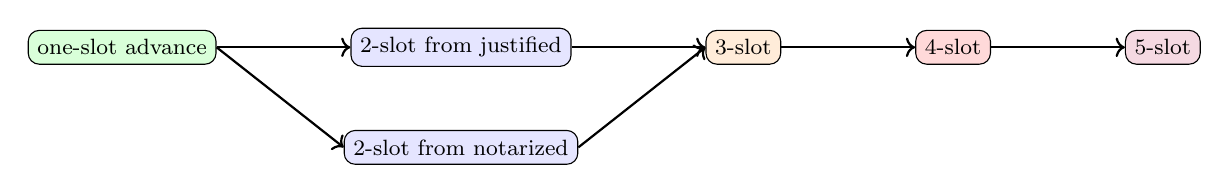
\begin{tikzpicture}[every node/.style={font=\footnotesize}, node distance=1.7cm]
  \node[draw, rounded corners, fill=green!15] (one) {one-slot advance};
  \node[draw, rounded corners, fill=blue!10, right=of one] (twoj) {2-slot from justified};
  \node[draw, rounded corners, fill=blue!10, below=8mm of twoj] (twon) {2-slot from notarized};
  \node[draw, rounded corners, fill=orange!15, right=of twoj] (three) {3-slot};
  \node[draw, rounded corners, fill=red!15, right=of three] (four) {4-slot};
  \node[draw, rounded corners, fill=purple!15, right=of four] (five) {5-slot};
  \draw[->, thick] (one.east) -- (twoj.west);
  \draw[->, thick] (one.east) -- (twon.west);
  \draw[->, thick] (twoj.east) -- (three.west);
  \draw[->, thick] (twon.east) -- (three.west);
  \draw[->, thick] (three.east) -- (four.west);
  \draw[->, thick] (four.east) -- (five.west);
\end{tikzpicture}
\end{center}

\begin{lemma}[Healing: one-slot advance]\label{lem:healing-one-slot}
$f^{\vote(k+1)} < n/3$; $\start(k) - \Delta \geq \GST$; \OHM, \AHA at $k$; honest \getConfirmed{}'s at $\vote(k)$ are pairwise compatible at common state-height $\comm{h}$; no honest has cast at height $\geq \comm{h}$ before $\vote(k)$. Then the system is healed at slot $k+1$ with height $\comm{h}$.
\end{lemma}

\begin{proof}[Sketch] Every honest casts slot-$k$ R1 \just{} at height $\comm{h}$ on the common chain $C$. By synchrony, all such votes are delivered to every honest by $\vote(k+1)$. The virtual-block aggregation fires a same-slot cert at height $\comm{h}$ on $C$: bit-1 if all honest \jtargets coincide, bit-0 at the prefix-notar $\arg\max$ otherwise. The dishonest-only quorum bound rules out cert events above $\comm{h}$. So $R_v^{\vote(k+1)}.h = \comm{h}$ uniformly with cert-key slot $k = (k+1)-1$ when bit 0. The healed-state conditions follow. \end{proof}

\begin{lemma}[Two-slot healing from a justified common root]\label{lem:healing-from-justified}
\OHM at $k, k+1$; \AHA at $k, k+1$; \HAR at $k$; honest $R_v^{\vote(k)} = \comm{R}$ is a justified block at height $\comm{h}$; \getConfirmed{}'s pairwise compatible at common state-height $\comm{h}$; no honest at $> \comm{h}$ before $\vote(k)$. Then the system is healed at slot $k+2$ with height $\comm{h}+1$.
\end{lemma}

\begin{proof}[Sketch] At $\vote(k)$ every honest casts slot-$k$ R1 \just{} at height $\comm{h}$ on the common chain $D$. Slot-$k$ bit-0 same-slot cert at $\comm{h}$ fires in every honest's view by $\vote(k+1)$ but is dominated by the cached bit-1 (no $R$-update). \HAR + \AHA + the property of $\getConfirmed$ under stable root force the canonical state-height to advance to $\comm{h}+1$ by $\vote(k+1)$ (the slot-$k$ honest votes all land in $\getConfirmed_v^{\vote(k+1)}$). Then apply Lemma~\ref{lem:healing-one-slot} at slot $k+1$ with $\comm{h}' = \comm{h}+1$. \end{proof}

\begin{lemma}[Two-slot healing from a notarized common root]\label{lem:healing-from-notarized}
$\syncer(k+1)$ honest; \OHM, \AHA, \HAR conditions; honest $R_v^{\vote(k)}$ is a bit-0 notarized block at $\comm{h}$ for slot $k-1$. Then the system is healed at slot $k+2$ with height $\comm{h}+1$.
\end{lemma}

\begin{proof}[Sketch] Two cases at $\vote(k+1)$ via view-merge: a bit-1 cert at $\comm{h}$ has fired (reduce to Lemma~\ref{lem:healing-from-justified} at $k+1$) or not (reduce to a dedicated ``no-just-completing'' variant; the slot-$k$ same-slot bit-0 cert at $\comm{h}$ then dominates the cached bit-0 on $s_n$, lifting $R$ to a fresh slot-$k$ notarization on $D$). Either way, in two more slots we reach $\comm{h}+1$. \end{proof}

\begin{lemma}[Three-slot healing]\label{lem:healing-three-slot}
$\syncer(k+1), \syncer(k+2)$ honest; \OHM, \AHA, \HAR conditions; honest \getConfirmed{}'s pairwise compatible at common state-height $\comm{h}$; no honest at $> \comm{h}$ before $\vote(k)$. Then the system is healed at slot $k+3$ with height $\comm{h}+1$.
\end{lemma}

\begin{proof}[Sketch] At $\vote(k+1)$ honest stores share $\comm{\Sigma}^{\vote(k+1)}$ via view-merge. Two cases on $\comm{R}^{\vote(k+1)}$: justified at $\comm{h}$ $\rightarrow$ Lemma~\ref{lem:healing-from-justified} at $k+1$; bit-0 at $\comm{h}$ for slot $k$ $\rightarrow$ Lemma~\ref{lem:healing-from-notarized} at $k+1$. Both conclude at $k+3$ with $\comm{h}+1$. \end{proof}

The four-slot and five-slot lemmas chain similar reductions, splitting on the bit and slot of the common root at the next view-merge time. The five-slot lemma ends in a healed state at \emph{some} $k' \in \{k+3, k+4, k+5\}$.

\begin{figure}[H]
\centering
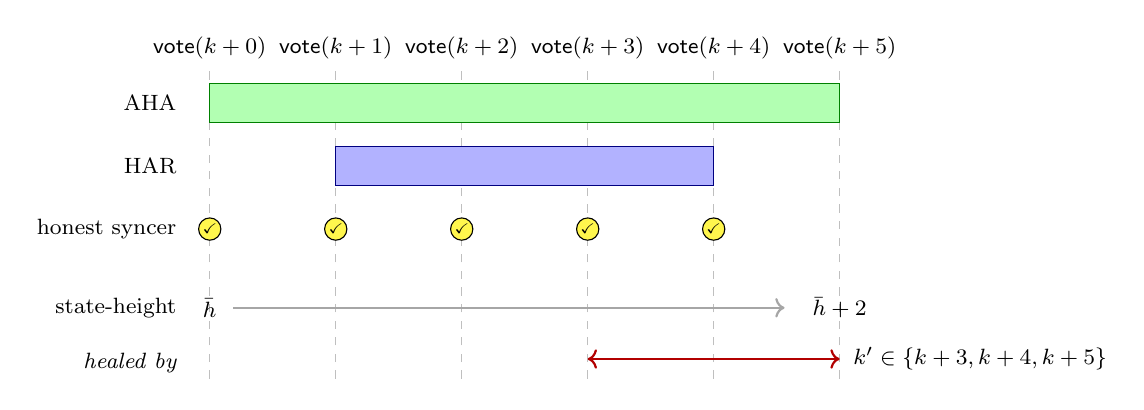
\begin{tikzpicture}[every node/.style={font=\footnotesize}]
  \foreach \i in {0,...,5} {
    \draw[gray!50, dashed] (\i*1.6, -2.2) -- (\i*1.6, 1.8);
    \node[font=\footnotesize] at (\i*1.6, 2.0) {$\vote(k+\i)$};
  }
  % AHA bar
  \node[anchor=east, font=\footnotesize] at (-0.3, 1.3) {AHA};
  \fill[green!30, draw=green!50!black] (0, 1.05) rectangle (8.0, 1.55);
  % HAR bar
  \node[anchor=east, font=\footnotesize] at (-0.3, 0.5) {HAR};
  \fill[blue!30, draw=blue!50!black] (1.6, 0.25) rectangle (6.4, 0.75);
  % Honest syncer markers
  \node[anchor=east, font=\footnotesize] at (-0.3, -0.3) {honest syncer};
  \foreach \i in {0,1,2,3,4} {
    \node[draw, circle, fill=yellow!70, inner sep=0.5pt, font=\tiny] at (\i*1.6, -0.3) {$\checkmark$};
  }
  % State-height progression
  \node[anchor=east, font=\footnotesize] at (-0.3, -1.3) {state-height};
  \node[font=\footnotesize] at (0, -1.3) {$\comm{h}$};
  \draw[->, thick, gray!70] (0.3, -1.3) -- (7.3, -1.3);
  \node[font=\footnotesize] at (8.0, -1.3) {$\comm{h}+2$};
  \node[anchor=east, font=\footnotesize\itshape] at (-0.3, -2.0) {healed by};
  \draw[<->, thick, red!70!black] (4.8, -1.95) -- (8.0, -1.95);
  \node[font=\footnotesize\itshape, anchor=west] at (8.05, -1.95) {$k' \in \{k+3, k+4, k+5\}$};
\end{tikzpicture}
\caption{Healing window. Five honest syncers, six AHA slots, four HAR slots: the system reaches a healed state at some $k' \in \{k+3, k+4, k+5\}$ with state-height $\comm{h}+2$, after which Lemma~\ref{lem:healing-unbounded} carries chain compatibility and monotonicity forward indefinitely.}\label{fig:healing-timeline}
\end{figure}

\subsection{Main healing theorem}

\begin{theorem}[Healing main theorem]\label{thm:healing-main}
Assume:
\begin{enumerate}
\item $f^{\vote(k+5)} < n/3$ and honest validators follow Definition~\ref{def:voting-rule};
\item $\start(k) - \Delta \geq \GST$;
\item $\syncer(k), \ldots, \syncer(k+4)$ are honest;
\item \OHM holds at every slot $k' \geq k+1$;
\item \AHA holds at slots $k, k+1, \ldots, k+5$;
\item \HAR holds at slots $k+1, k+2, k+3, k+4$;
\item $\sigma[\getConfirmed_v^{\vote(k)}].h = \comm{R}^{\vote(k)}.h$ is the same $\comm{h}$ for every honest $v$;
\item no honest validator has cast at height $> \comm{h}+1$ before $\vote(k)$.
\end{enumerate}
Then for every honest pair and every $t, t' \geq \vote(k+5)$:
\[
  \getConfirmed_v^t \sim \getConfirmed_{v'}^{t'}, \quad \text{and} \quad \getConfirmed_v^{t'} \succeq \getConfirmed_v^t \text{ when } t \leq t'.
\]
\end{theorem}

\begin{proof}[Sketch] The five-slot healing lemma yields a $k' \in \{k+3, k+4, k+5\}$ at which the system is healed at height $\comm{h}+2$. Lemma~\ref{lem:healing-unbounded} then propagates compatibility and monotonicity to all $t \geq \vote(k')$, hence to all $t \geq \vote(k+5)$. \end{proof}

\flag{The cascade above is presented as a clean recursion. In the original document the four/five-slot lemmas split on the cached cert-key state at the next view-merge time, and there are two distinct ``four-slot'' lemmas (from-justified and from-notarized). My sketch glosses over: (i)~the exact slot-$k$ cert-key configuration that distinguishes those branches; (ii)~the degenerate ``mixed state-height'' case at $\vote(k)$ in the four-slot-from-justified lemma, where some honest are at $\comm{h}$ and others at $\comm{h}+1$ and the proof has to land all of them at $\comm{h}+1$ before invoking the three-slot lemma.}

\subsection{Properties of \getConfirmed}\label{sec:gc-properties}

The healing arguments rely on four properties of $\getConfirmed$ under a stable root, treated as black-box assumptions on the auxiliary chain mechanism:

\begin{property}[Target compatibility]\label{prop:gc-compat}
Under synchrony, \OHM, common honest roots at $\vote(k)$, and the existence of an honest $v_\ell$ with $\getConfirmed_{v_\ell}^{\vote(k)} \succeq R_v^t$ for every honest $v$ and $t \in [\vote(k), \vote(k+1)]$: honest \getConfirmed's are pairwise compatible across the interval.
\end{property}

\begin{property}[Target monotonicity under stable root]\label{prop:gc-mono} Same hypotheses: honest \getConfirmed's are monotone within the interval. \end{property}

\begin{property}[Honest-vote inclusion]\label{prop:gc-inclusion} Same hypotheses + \HAR: every slot-$k$ honest vote is included on the chain ending at $\getConfirmed_v^{\vote(k+1)}$ for every honest $v$. \end{property}

\begin{property}[Target dominance]\label{prop:gc-dominance} Same hypotheses + \HAP: $\getConfirmed_v^{\vote(k+1)} \succeq \getConfirmed_{v_\ell}^{\vote(k)}$ for every honest $v$. \end{property}

\paragraph{Why these are properties, not lemmas.} They abstract over the available-chain mechanism (the $\Omega$ argument of \getConfirmed) and the propose-and-relay layer. The finality gadget is correct conditional on them; their proofs are part of the underlying available-chain protocol (Simplex / etc.).

\appendix
\section{View-merge mechanism}\label{app:view-merge}

The view-merge protocol is one concrete realization of Definition~\ref{ass:view-merge}.

\begin{definition}[Slot timing]\label{def:slot-timing}
Each slot $k$ has start time $\start(k)$ with $\start(k+1) - \start(k) \geq 2\Delta$. Three events:
\begin{itemize}
\item \emph{Freeze} at $\start(k) - \Delta$: every validator $i$ records its current store as $\Sigma^k_{\mathrm{frozen}, i}$.
\item \emph{Syncer} at $\start(k)$: $\syncer(k)$ broadcasts its current store $\Sigma^k_{\mathrm{sent}}$.
\item \emph{Vote} at $\start(k) + \Delta$: every honest $i$ invokes Definition~\ref{def:voting-rule} on the merged view $\Sigma^k_{\mathrm{merge}, i} = \Sigma^k_{\mathrm{frozen}, i} \cup \Sigma^k_{\mathrm{sent}}$.
\end{itemize}
\end{definition}

\begin{definition}[Synchronous slot]\label{def:sync-slot}
Slot $k$ is \emph{synchronous} if every message sent in $[\start(k) - 2\Delta, \start(k) + \Delta]$ is delivered within $\Delta$ of its sending time.
\end{definition}

\begin{lemma}[View-merge under honest synchronous syncer]\label{lem:view-merge}
If slot $k$ is synchronous and $\syncer(k)$ is honest, then every honest $i$ has $\Sigma^k_{\mathrm{merge}, i} = \Sigma^k_{\mathrm{sent}}$, discharging Definition~\ref{ass:view-merge}.
\end{lemma}

\begin{proof}[Proof]
Any message in $\Sigma^k_{\mathrm{frozen}, i}$ was received by $\start(k) - \Delta$, hence sent by then, hence delivered to $\syncer(k)$ by $\start(k)$ under synchrony --- so it lies in $\Sigma^k_{\mathrm{sent}}$. The broadcast at $\start(k)$ reaches every honest by $\start(k) + \Delta$, so the merged view equals $\Sigma^k_{\mathrm{sent}}$.
\end{proof}

\hrule\medskip

\paragraph{Summary of flags.} Two simplifications above are flagged: (1)~the persistence-over-one-slot proof is collapsed from a 3-case $\times$ 2-sub-case analysis to three top-level cases (\S\ref{sec:cascade}); (2)~the cascade glosses over the slot-$k$ cert-key configuration that distinguishes the two four-slot variants (Theorem~\ref{thm:healing-main}). Both are faithful at the level of the main argument; for the exact case bookkeeping see the original document.

The original also contains, post-Theorem~\ref{thm:healing-main}, a dual-height-voting variant lemma annotated by the authors as ``proof not checked.'' That lemma is omitted here.

\end{document}
